	\documentclass[aspectratio=43]{beamer}
\usepackage[english]{babel}
\usepackage{amsthm}
\usepackage{amsfonts}
\usepackage{amsmath}
\usepackage{amssymb}
\usepackage{mathtools}
\usepackage{bbm}
\usepackage{pgfplots}
\usepackage{tikz}
%\usepackage{physics}
\usepackage{calligra}
\usepackage{csquotes}
%\usepackage{tensor}
\usepackage[thicklines]{cancel}
\usepackage{tcolorbox}
%\usepackage{pstricks}
\usepackage[backend=biber, bibstyle=nature, sorting=nty, citestyle=numeric-comp]{biblatex} %Custom bibliography
    \addbibresource{bib.bib} %Load references
\usepackage{chronology}
\usepackage{msc}

\DeclareMathAlphabet{\mathcalligra}{T1}{calligra}{m}{n}
\DeclareFontShape{T1}{calligra}{m}{n}{<->s*[2.2]callig15}{}
\newcommand{\scriptr}{\mathcalligra{r}\,}
\newcommand{\boldscriptr}{\pmb{\mathcalligra{r}}\,}
\def\rc{\scriptr}
\def\brc{\boldscriptr}
\def\hrc{\hat\brc}
\newcommand{\ie}{\emph{i.e.}} %id est
\newcommand{\eg}{\emph{e.g.}} %exempli gratia
\newcommand{\rtd}[1]{\ensuremath{\left\lfloor #1 \right\rfloor}}
\newcommand{\dirac}[1]{\ensuremath{\delta \left( #1 \right)}}
\newcommand{\diract}[1]{\ensuremath{\delta^3 \left( #1 \right)}}
\newcommand{\e}{\ensuremath{\epsilon_0}}
\newcommand{\m}{\ensuremath{\mu_0}}
\newcommand{\V}{\ensuremath{\mathcal{V}}}
\newcommand{\prnt}[1]{\ensuremath{\left(#1\right)}} %parentheses
\newcommand{\colch}[1]{\ensuremath{\left[#1\right]}} %square brackets
\newcommand{\chave}[1]{\ensuremath{\left\{#1\right\}}}  %curly brackets
\newcommand\eqdef{\stackrel{\mathclap{\normalfont \tiny\mbox{\textrm{def}}}}{=}}
\useoutertheme{infolines}
\useinnertheme{rectangles}
\usefonttheme{professionalfonts}


\definecolor{blue2}{HTML}{045FB4}
\definecolor{green2}{HTML}{46C235}
\definecolor{red2}{HTML}{EE4848}
\definecolor{violet2}{HTML}{A647E5}
\definecolor{orange2}{HTML}{FF7425}
\definecolor{darkred}{HTML}{5C2020}
\definecolor{gray}{HTML}{303030}
\definecolor{yellow}{HTML}{f0be52}
\definecolor{lightdarkgold}{HTML}{EEBC1D}

\renewcommand{\CancelColor}{\color{darkred}}

\makeatletter
\newcommand{\mybox}[1]{%
  \setbox0=\hbox{#1}%
  \setlength{\@tempdima}{\dimexpr\wd0+13pt}%
  \begin{tcolorbox}[colback=gray,colframe=gray,boxrule=0.5pt,arc=4pt,
      left=6pt,right=6pt,top=6pt,bottom=6pt,boxsep=0pt,width=\@tempdima]
    \textcolor{yellow}{#1}
  \end{tcolorbox}
}
\makeatother


\pgfplotsset{my style/.append style={axis x line=middle, axis y line=
middle, xlabel={$x$}, ylabel={$y$}, axis equal }}


\usecolortheme[named=gray]{structure}
\usecolortheme{sidebartab}
\usecolortheme{orchid}
\usecolortheme{whale}
\setbeamercolor{titlelike}{parent=structure, bg=structure, fg=white}
\setbeamercolor{section in toc}{fg= white}
\setbeamercolor{subsection in toc}{fg= white}
%\setbeamercolor*{sidebar}{fg=red2,bg=gray!15!white}

\setbeamercolor{item projected}{bg=yellow, fg = gray}
\setbeamertemplate{enumerate items}[default]
\setbeamertemplate{navigation symbols}{}
\setbeamercolor{local structure}{fg=yellow}

\setbeamercolor{alerted text}{fg=white}
\setbeamercolor{block title}{bg = yellow}
\setbeamercolor{block title alerted}{bg=red2}
\setbeamercolor{block title example}{bg=green2}
\setbeamercolor{background canvas}{bg=gray}
\setbeamercolor{normal text}{bg=gray,fg=white}


\setbeamertemplate{footline}
        {
      \leavevmode%
      \hbox{%
      \begin{beamercolorbox}[wd=.333333\paperwidth,ht=2.25ex,dp=1ex,center]{author in head/foot}%
        \usebeamerfont{author in head/foot}\insertshortauthor~~(\insertshortinstitute)
      \end{beamercolorbox}%
      \begin{beamercolorbox}[wd=.333333\paperwidth,ht=2.25ex,dp=1ex,center]{title in head/foot}%
        \usebeamerfont{title in head/foot}\insertshorttitle
      \end{beamercolorbox}%
      \begin{beamercolorbox}[wd=.333333\paperwidth,ht=2.25ex,dp=1ex,center]{date in head/foot}%
        \usebeamerfont{date in head/foot}\insertshortdate{}%\hspace*{2em}

    %#turning the next line into a comment, erases the frame numbers
        %\insertframenumber{} / \inserttotalframenumber\hspace*{2ex} 

      \end{beamercolorbox}}%
      \vskip0pt%
    }


\setbeamertemplate{blocks}[rectangle]
\setbeamercovered{dynamic}




%\setbeamercolor{author}{fg=yellow}
%\setbeamercolor{title}{fg = yellow}
%\setbeamerfont{title}{size=\Large, series=\bfseries}
%\setbeamerfont{author}{size=\footnotesize}
%\setbeamerfont{date}{size=\small}


\setbeamertemplate{section page}
{
	\begin{centering}
		\begin{beamercolorbox}[sep=27pt,center]{part title}
			\usebeamerfont{section title}\insertsection\par
			\usebeamerfont{subsection title}\insertsubsection\par
		\end{beamercolorbox}
	\end{centering}
}





%\setbeamertemplate{subsection page}
%{
%	\begin{centering}
%		\begin{beamercolorbox}[sep=12pt,center]{part title}
%			\usebeamerfont{subsection title}\insertsubsection\par
%		\end{beamercolorbox}
%	\end{centering}
%}

\newcommand{\hlight}[1]{\colorbox{violet!50}{#1}}
\newcommand{\hlighta}[1]{\colorbox{darkred!50}{#1}}


    \setbeamertemplate{background} 
    {
        
\includegraphics[width=\paperwidth,height=\paperheight]{images/fond1.jpg}
    }
\title{Hack the Web3.0 : SDK3 for Web3} %->->->->-> Check hyperref title <-<-<-<-<-
\subtitle{ZKP Tools in the Nano}
\author[R. Dubois]{\textcolor{yellow}{Renaud Dubois}}
\institute[LIT]{
    \textcolor{white}{Ledger}%
    \\%
    \textcolor{white}{Innovation Team}%
} %You can change the Institution if you are from somewhere else
\date{\today}
%\logo{\includegraphics[width= 0.05\textwidth]{images/logo.png}}

\begin{document}
    
    \frame{\titlepage}
    
%%%%%%%%%%%%%%%%%%%%%%%%%%%%%%%%%%%%%%%%%%%%%%%%%%%%%%%%%%%%%%%%%%%%%%%%%% 
\section{ZKP : The Epic Fight between Snarks and Starks}
 

\begin{frame}
 \begin{center}
    
 \begin{tabular}{|ccc|} 
\hline
 STARKs & & SNARKs\\
 
 
\includegraphics[width=3.5cm]{images/stark.jpg}
  &
  \huge{\bf VS}
  &~~~
 
\includegraphics[width=3cm]{images/snark.jpg}~~~\\
 \hline
 Computational integrity  & & Privacy-enhancing\\
 \hline
 Post quantum, No trusted Setup && Asymptotic complexities ++ \\
 \hline
 Delegation, Layer 2 && SSI, transaction hiding \\
 \hline
 \end{tabular}
 \end{center}
 
 \only<2>{
 Snarks are fun because they used Pairings. And Pairings are cool.
 }
 
\end{frame}

%%%%%%%%%%%%%%%%%%%%%%%%%%%%%%%%%%%%%%%%%%%%%%%%%%%%%%%%%%%%%%%%%%%%%%%%%% 
\section{Zero Knowledge Proofs}

\begin{frame}
 \begin{center}
 \textcolor{yellow}{\fbox{Zero Kowledge Proofs}} 
 \end{center}
 
 

 \fbox{\parbox{\textwidth}{

 \begin{itemize} 
 
 \item Pairings enable Zk-snarks, Commitments, Efficient signatures
 \item Ledger direct examples : Linkable Signatures for Anonymous airdrop ({\bf device ID}), Ring signature ({\bf endorsement}), Strongly Verifiable SS ({\bf Protect}), {\bf Decentralized Identifiers}.
 \item More info : 
 \begin{itemize} 
 \item \url{https://github.com/rdubois-crypto/PrivacyProtocols/blob/main/report/Privacy.pdf}
 \end{itemize}
 \end{itemize}
 
 }}
 \vskip+1cm
All of this provides futurist SSI and DIds systems, and endpoint needs to implement Pairings for efficiency.

\end{frame}

%%%%%%%%%%%%%%%%%%%%%%%%%%%%%%%%%%%%%%%%%%%%
\begin{frame}
 
 
 \only<1>{
 \begin{center}
 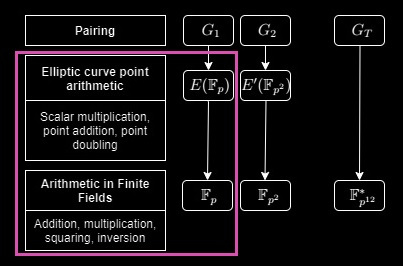
\includegraphics[width=7cm]{cryptomodules2.jpg}
 \end{center}
 
 
 \begin{center}
 \textcolor{yellow}{\fbox{The Initial Hack Objective}} 
 \fbox{\parbox{\textwidth}{

 \begin{itemize} 
 \item Strip modular arithmetic from Open Source (blst library)
 \item Accelerate using bolos calls (available in pink square on figure)
 \item Push the result as a ``Package'' that external developpers can use for ZKP integration on Nano.
 \item https://github.com/rdubois-crypto/hackthew3
 \end{itemize}
 }}
 }
 \only<2-3>{
 \begin{center}
 \textcolor{yellow}{\fbox{What did we achieve ?}}
 \vskip+0.5cm
 \fbox{\parbox{\textwidth}{
\only<2>
{
 \begin{center}
 
 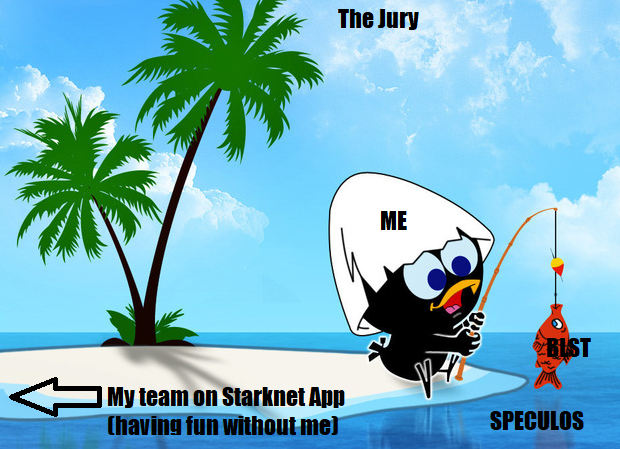
\includegraphics[width=7cm]{images/calimero.png}
 \end{center}
 
 Not much : alone, no Montgomery handling yet in speculos
 
}
\only<3>{
 \begin{itemize} 
 \item Blst deep understanding, capacity to wrap efficiently
 \item Identification of source code ``strip-required points''
 \item Integrate blst for ``speculos-pairing ready version''
 \item https://github.com/rdubois-crypto/hackthew3
 \end{itemize}
 }}}
 
 
 }
 \end{center}
 
 
\end{frame}

%%%%%%%%%%%%%%%%%%%%%%%%%%%%%%%%%%%%%%%%%%%%%%%%%%%%%%%%%%%%%%%%%%%%%%%%%%
    \section{}
    \begin{frame}{}
        \centering
            \Huge\bfseries
        \textcolor{yellow}{Questions ?}
            
\includegraphics[width=12cm]{images/questions.jpg}
     
    \end{frame}
\end{document}

% https://en.wikipedia.org/wiki/Privacy
% [CL16]: Concepts Around Privacy-Preserving Attribute-Based CredentialsJan Camenisch  https://hal.archives-ouvertes.fr/hal-01276046/document
